% Asset ID: AS1GraphsTransformationsTikZ-005
% Source: CCEA AS1-AF-LO016 + DrFrost transformation summary transcript
% Purpose: Summarise simple transformations of y=f(x)
\documentclass[tikz,border=8pt]{standalone}
\usepackage{amsmath}
\usetikzlibrary{arrows.meta,positioning,shapes.geometric}
\begin{document}
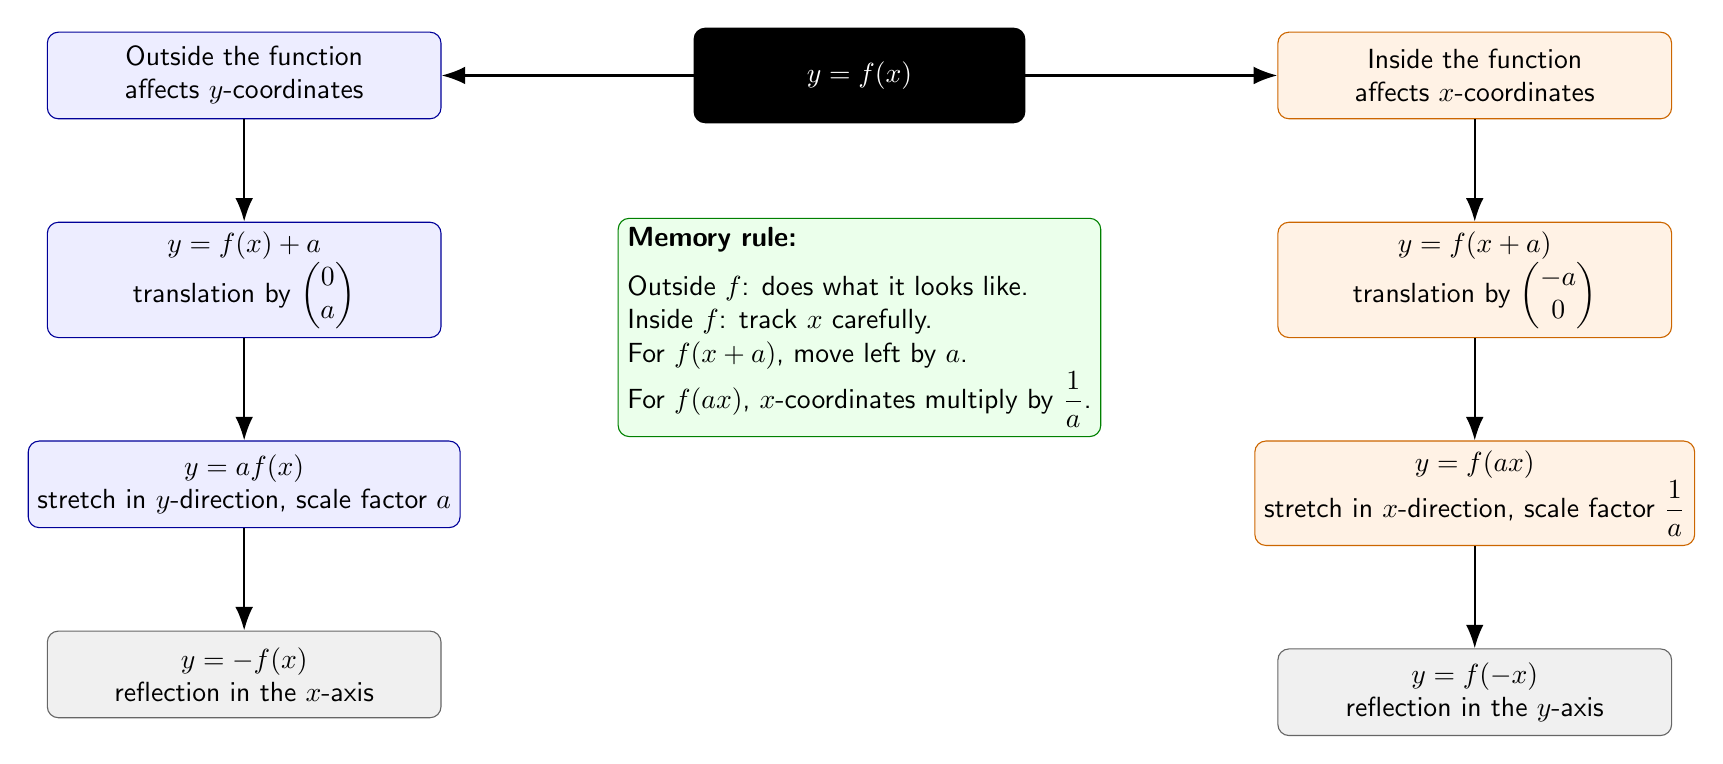
\begin{tikzpicture}[node distance=1.3cm and 1.2cm,every node/.style={font=\sffamily},hub/.style={rectangle,rounded corners,draw=black,fill=black,text=white,minimum width=4.2cm,minimum height=1.2cm,align=center,font=\sffamily\bfseries},outside/.style={rectangle,rounded corners,draw=blue!60!black,fill=blue!7,minimum width=5cm,minimum height=1.1cm,align=center},inside/.style={rectangle,rounded corners,draw=orange!80!black,fill=orange!10,minimum width=5cm,minimum height=1.1cm,align=center},reflection/.style={rectangle,rounded corners,draw=gray!80!black,fill=gray!12,minimum width=5cm,minimum height=1.1cm,align=center},note/.style={rectangle,rounded corners,draw=green!50!black,fill=green!8,minimum width=5.5cm,align=left},arrow/.style={-{Latex[length=3mm]},thick}]
\node[hub](start){$y=f(x)$};
\node[outside,left=3.2cm of start](outside){Outside the function\\affects $y$-coordinates};
\node[outside,below=of outside](updown){$y=f(x)+a$\\translation by $\begin{pmatrix}0\\a\end{pmatrix}$};
\node[outside,below=of updown](ystretch){$y=af(x)$\\stretch in $y$-direction, scale factor $a$};
\node[reflection,below=of ystretch](xreflect){$y=-f(x)$\\reflection in the $x$-axis};
\node[inside,right=3.2cm of start](inside){Inside the function\\affects $x$-coordinates};
\node[inside,below=of inside](leftright){$y=f(x+a)$\\translation by $\begin{pmatrix}-a\\0\end{pmatrix}$};
\node[inside,below=of leftright](xstretch){$y=f(ax)$\\stretch in $x$-direction, scale factor $\dfrac1a$};
\node[reflection,below=of xstretch](yreflect){$y=f(-x)$\\reflection in the $y$-axis};
\draw[arrow](start)--(outside);\draw[arrow](start)--(inside);\draw[arrow](outside)--(updown);\draw[arrow](updown)--(ystretch);\draw[arrow](ystretch)--(xreflect);\draw[arrow](inside)--(leftright);\draw[arrow](leftright)--(xstretch);\draw[arrow](xstretch)--(yreflect);
\node[note,below=1.2cm of start](memory){\textbf{Memory rule:}\\[2mm]Outside $f$: does what it looks like.\\Inside $f$: track $x$ carefully.\\For $f(x+a)$, move left by $a$.\\For $f(ax)$, $x$-coordinates multiply by $\dfrac1a$.};
\end{tikzpicture}
\end{document}
